\section{The Particle Tracking Algorithm}
\label{sec:particleTrackingAlgo}

The particle tracking algorithm used in OpenFOAM was published in \cite{macpherson08}. Since it is crucial for the optimization it is presented here.

\subsection{Basic Particle Tracking Algorithm}

\begin{figure}[H]
  \centering
  \begin{tikzpicture}

% Coords of the Axes
\coordinate (Zero)  at (0,0);
%\coordinate [label=below:$x$](Xend)  at (10,0);
%\coordinate [label=right:$y$](Yend)  at (0,10);

% Coords for cell A
\coordinate (f1start) at (0.5,2);
\coordinate (f1end) at (12,3);
\coordinate (f2start) at (10,1);
\coordinate (f2end) at (11,8);
\coordinate (f3start) at (12,7);
\coordinate (f3end) at (1,8);
\coordinate (f4start) at (3,9);
\coordinate (f4end) at (1,1);

% Intersection between the cell faces: k, l, m, n
% Syntax note: Do NOT make a space between the coord and the --!
% Bottom left
\coordinate (k) at (intersection of f1start--f1end and f4start--f4end);
% Bottom right
\coordinate [label={below right:cell b}] 
	(l) at (intersection of f1start--f1end and f2start--f2end);
% Top right
\coordinate [label={below left:cell a},label={below right:cell c}]  
	(m) at (intersection of f2start--f2end and f3start--f3end);
% Top left
\coordinate (n) at (intersection of f3start--f3end and f4start--f4end);

% Add the face indexes, note that only coordinates and nodes can have labels
\coordinate [label=below:$0$] (0) at ($ (k)!.5!(l) $);
\fill[black] (0) circle (2pt);
\coordinate [label=left:$1$, label={below right:$\mathbf{C_f}$}] 
	(1) at ($ (l)!.5!(m) $);
\fill[black] (1) circle (2pt);
\coordinate [label=above:$2$] (2) at ($ (m)!.5!(n) $);
\fill[black] (2) circle (2pt);
\coordinate [label=left:$3$] (3) at ($ (n)!.5!(k) $);
\fill[black] (3) circle (2pt);

% Centroid
\coordinate (sum) at  ($ (k)+(l)+(m)+(n) $);
\coordinate [label=left:$\mathbf{C_c}$] (Cc) at ($ 1/4*(sum) $);
\fill[black] (Cc) circle (2pt);

% Draw the lines, which define cell A, B and C
%\draw [thin,->] (Zero) -- (Xend);
%\draw [thin,->] (Zero) -- (Yend);
\draw (f1start) -- (f1end);
\draw (f2start) -- (f2end);
\draw (f3start) -- (f3end);
\draw (f4start) -- (f4end);

% Cf
\coordinate[label=right:$\vec{S_f}$] (S) at ($(1)!0.5! -90:(m)$);
\draw [->,dashed] (1) -- (S);

% Particle movement
\coordinate[label=right:$\textbf{a}$] (a) at (8,6);
\coordinate[label=right:$\textbf{b}$] (b) at (12,2);

\coordinate[label=right:$\textbf{p}$] (p) at 
	(intersection of a--b and f2start--f2end);
\coordinate[label=above:$\textbf{p'}$] (p_) at 
	(intersection of a--b and f1start--f1end);

\draw[fill=white,thick,->] (a) -- (b);

\draw[fill=white,dashed,->] (Cc) -- (b);

\filldraw[fill=white] (a) circle (2pt);
\filldraw[fill=white] (p) circle (2pt);
\filldraw[fill=white] (p_)circle (2pt);
\filldraw[fill=white] (b) circle (2pt);

\end{tikzpicture}
  \caption{Example situation in two dimensions illustrates the particle tracking algorithm.}
  \label{fig:f2f}
\end{figure}

For the Lagrangian-Eulerian coupling it is required to know, for every time step, which cells a particle crosses and how much time it spent there. Figure \ref{fig:f2f} illustrates the particle tracking algorithm during a time step. The particle is initially located at position $\vec{a}$ and moves to $\vec{b}$. While traveling along the straight line from $\vec{a}$ to $\vec{b}$ it changes the cell twice at $\vec{p}$ and $\vec{p'}$.

The point where the particle hits the face is calculated by the following equation:

\begin{equation}
  \label{eq:1}
  \vec{p} = \vec{a} + \lambda_a \cdot (\vec{b}-\vec{a})
\end{equation}

$\lambda_a$ denotes the fraction of the path vector which the particle travels until it hits the first face (the distance from $\vec{a}$ to $\vec{p}$). In this equation $\lambda_a$ and $\vec{p}$ are unknown, we only know the start and end position of the particle ($\vec{a}$ and $\vec{b}$). The vector from $\vec{C_f}$ to $\vec{p}$ along the face is orthogonal to the face normal. This leads to the definition of another equation, which can be used to calculate $\vec{p}$:

\begin{equation}
 \label{eq:2}
 (\vec{p} - \vec{C_f}) \bullet \vec{S_f} = 0
\end{equation}

In the equation above we used the fact that the dot product of two orthogonal vectors is zero. Now substituting equation (\ref{eq:1}) into equation (\ref{eq:2}) and solving for $\lambda_a$ gives:

\begin{equation}
  \label{eq:3}
  \lambda_{a} = \frac{(\vec{C_f} - \vec{a}) \bullet \vec{S_f}}
                       {(\vec{b} - \vec{a}) \bullet \vec{S_f}}
\end{equation}

Now since $\vec{p}$ no longer appears in equation (\ref{eq:3}) we can calculate $\lambda_{a}$ for each face respective of the cell. The face with the smallest $\lambda_{a} \in [0, 1]$ is the face, which is crossed by the particle. The particle is then moved along the line from $\vec{a}$ to $\vec{b}$ onto the face hit i.e. $\vec{p} = \vec{a} + \lambda_a \cdot (\vec{b} - \vec{a})$. The particles's occupancy information is updated to the cell on the other side of the face. The next tracking event works in the same way as the one just presented. This is repeated until the whole time step is processed. If $\lambda_{a}$ is not in the interval $[0,1]$, then the particle's end position $\vec{b}$ must be inside the same cell.

\subsection{Modified Tracking Algorithm}

If a face is defined by more than three vertices, then these do not necessarily lie in a plane. In case a face is non-planar the mesh stores the face centroid and interpolates a normal vector which represents the effective plane of the face. When using the effective planes as cell faces, the cells in a mesh are no longer space-filling! It is therefore possible to loose track of a particle when it crosses a face close to a vertex. The deficiencies of the basic particle tracking algorithm are further described in \cite[page 267]{macpherson08}.  While these deficiencies seem to appear in rather large non-standard cases it should be mentioned that the modified tracking algorithm also solves a simple implementation problem of the basic particle algorithm: Just naively moving the particle onto the face hit and then evaluate the formula for $\lambda_a$ again for the new occupancy cell may yields the same face again as before, depending on how the dices of floating point accuracy roll. The problem can be solved by moving the particle just a little bit more into the next cell using an $\epsilon$-environment or by disabling the face in the subsequent calculation\footnote{In the authors experience the first solution, using an $\epsilon$-environment did not work in all cases, it was necessary to disable the face hit for the next calculation.}. There is no such problem when using the modified tracking algorithm, since the cell centre is taken as reference point inside the cell and not the particles actual position in order to get a list of faces which might be hit by the particle.

With reference to figure \ref{fig:f2f}, instead of taking the starting point of a particle, the cell centre is taken as reference point inside the cell to determine which faces the particle may crosses (if any). Replacing $\vec{a}$ with $\vec{C_c}$ in equation (\ref{eq:3}) gives:

\begin{equation}
  \label{eq:4}
  \lambda_{c} = \frac{(\vec{C_f} - \vec{C_c}) \bullet \vec{S_f}} 
                       {(\vec{b} - \vec{C_c}) \bullet \vec{S_f}}
\end{equation}

The line from $\vec{C_c}$ to $\vec{b}$ (shown dashed in figure \ref{fig:f2f}) crosses face 1 and 0\footnote{Or more precisely the plane which is defined by the face normal of face 0.}. Equation (\ref{eq:4}) therefore yields $\lambda_{c}$ between 0 and 1 for face 0 and face 1. If there is no face with  $\lambda_{c} \in [0,1]$, then $\vec{b}$ must be in the same cell as $\vec{a}$. Otherwise it is also necessary to calculate $\lambda_{a}$ using equation (\ref{eq:3}) for the faces, which are crossed by the line from $\vec{C_c}$ to $\vec{b}$ (face 0 and 1 in this case). The lowest value of $\lambda_{a}$ determines then which face was actually hit and the fraction of the time step, which it took to travel to the face can be determined using $\lambda_{a}$. The cell occupancy is changed to the neighbouring cell of the face which was crossed (c in this case). With $\lambda_m = min(1,max(0,\lambda_{a}))$ equation (\ref{eq:moveParticleModified}) is then used to move the particle to p.

\begin{equation}
	\label{eq:moveParticleModified}
	\vec{p} = \vec{a} + \lambda_m \cdot ( \vec{b} - \vec{a} )
\end{equation} 

The complete tracking algorithm is shown below as pseudo code. This was taken from \cite{macpherson08} (algorithm 1).

\begin{algo}{Complete tracking algorithm}
\label{alg:ttf}

	\textbf{while} the particle has not yet reached its end position at $\vec{b}$ \textbf{do}
	
	\noindent\hspace*{1cm}find the set of faces, $F_i$ for which $0 \leq \lambda_c \leq 1$
	
	\noindent\hspace*{1cm}\textbf{if} size of $F_i=0$ \textbf{then}
	
	\noindent\hspace*{2cm}move the particle to the end position
	
	\noindent\hspace*{1cm}\textbf{else}
	
	\noindent\hspace*{2cm}find face $f \in F_i$ for which $\lambda_a$ is smallest
	
	\noindent\hspace*{2cm}move the particle according to equation \ref{eq:moveParticleModified} using this value of $\lambda_a$.
	
	\noindent\hspace*{2cm}set particle cell occupancy to neighbouring cell of face $f$
	
	\noindent\hspace*{1cm}\textbf{end if}

\textbf{end while}

\end{algo}

\subsection{Implementation in OpenFOAM (solidParticle Library)}

The actual implementation of the particle tracking algorithm is more complicated. In the example presented to explain the particle tracking algorithm (figure \ref{fig:f2f}) the velocity of the particle was assumed to be constant during the whole tracking step. In the \verb+solidParticle+ library the velocity of the particle is coupled to the velocity of the fluid: A drag model is used, which calculates the drag issued by the fluid phase onto the particle, assuming spherical particles. In other words the velocity of the particle depends on the velocity of the cell in which it resides and therefore the velocity changes once the particle changes the cell. Therefore, it is required to distinguish between Eulerian and Lagrangian time steps.

\begin{figure}[H]
  \centering
  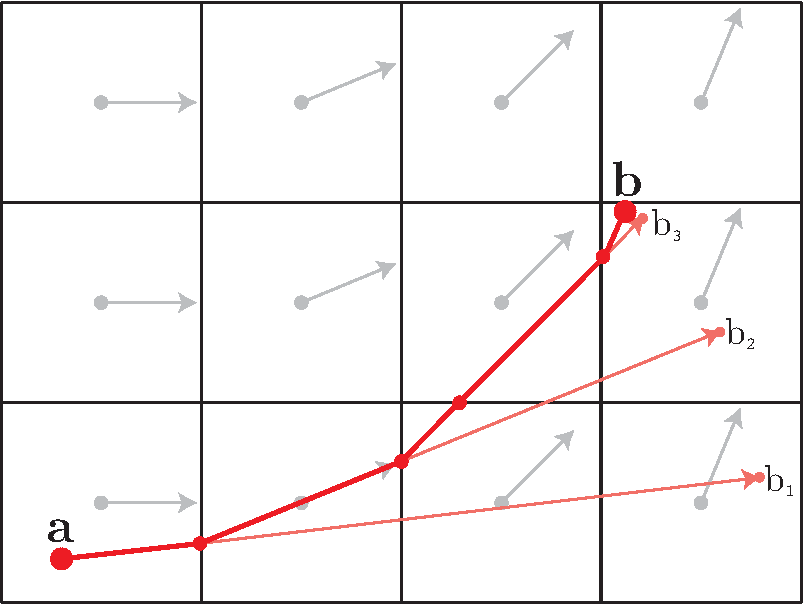
\includegraphics[scale=0.5]{content/gfx/lagrangianSteps.pdf}
  \caption{Two dimensional illustration of a particle trajectory through multiple cells.}
  \label{gfx:lagrangianSteps}
\end{figure}

Figure \ref{gfx:lagrangianSteps} shows a particle which starts at the beginning of a time step at position $\vec{a}$. Its end position is estimated using the velocity field in the cell in which point $\vec{a}$ lies. It is marked as $\vec{b_1}$ in figure 4. After changing the cell the first time, the end position is re-estimated using the velocity field in the new cell. This way the Eulerian time step is broken up into several smaller Lagrangian steps (5 in this example). The thick red line shows the actual trajectory of the particle. The light-red arrows show the estimated end position at the concerning sub steps.

The drag model used to calculate the velocity of the particles in the solidParticle library takes only drag and buoyancy forces into account.

\begin{equation}
    \label{eq:solidParticleVelocity}
    \frac{d \vec{U_p}}{dt} = D_c \cdot | \vec{U_{c}} - \vec{U_{p}} |
        + (1 - \frac{\rho_c}{\rho_p}) \cdot \vec{g}
\end{equation}

Here $\vec{U_p}$ is the velocity of the particle. $\vec{U_c}$ the velocity of the cell in which the particle resides, $\rho_p$ and $\rho_c$ are the densities for the particle and the fluid respectively. The drag coefficient $D_c$ is calculated using the Schiller-Naumann approximation \cite{schillerNaumann}.

\begin{equation}
    \label{eq:solidParticleDrag}        
    D_c = \frac{18}{d^2} \cdot \nu_c \cdot \frac{\rho_c}{\rho_p} 
        \cdot (1 + 0.15 \cdot Re_p^{0.687})
\end{equation}

Here $d$ is the diameter of the particle. The Reynolds number is calculated using the diameter is used $d$ as the characteristic length.

\begin{equation}
    \label{eq:solidParticleRe}
    Re_p = \frac{d}{\nu_c} \cdot | \vec{U_c} - \vec{U_p} |
\end{equation}
